% ch12b —— 中島啓「ミラー対称性を越えて」后半（PDF p.164-171 / 原书 p.156-163）
% 前半（PDF p.157-163 / 原书 p.149-155）在 ch12.tex，由 tr1 负责；本文件不写章标题与作者行，也不设置节号。
% 衔接：ch12.tex 已把「2 の不変量は 2'. …」这句补完（到条目 2'. 为止），本文件从锥形流形跃迁那句原文接写。
% ===== PDF p.164 (原书 p.156) =====
而且，我们预测：通过锥形流形跃迁，$L$ 的余法丛会定出锥形流形奇点消解之中的 Lagrangian 子流形 $\mathcal{L}_L$。$L$ 的余法丛是 $T^*S^3$ 中的 Lagrangian 子流形，而按这一预测，它经锥形流形跃迁之后也会以某种自然的方式搬过去。于是，代替 3，考虑

\noindent\textbf{3$'$．}\quad 从带边黎曼面到锥形流形奇点消解的全纯映射所得、且边界落入 $\mathcal{L}_L$ 的 Gromov--Witten 不变量

我们的主张是：它与 2$'$ 的不变量相等，因而也与链环 $L$ 的 Jones--Witten 不变量相等。这一猜想要从带边黎曼面出发考虑全纯映射，而 $\mathcal{L}_L$ 的定义又尚不明确，所以它还不是数学上可以严格验证的猜想。不过，对特殊的链环，在相当合理的 $\mathcal{L}_L$ 定义、以及用环面作用定义的 Gromov--Witten 不变量之下，人们已经做过计算并得到验证。

\section{几何工程——geometric engineering}

前一节把 Gromov--Witten 不变量与实 3 维拓扑不变量联系了起来。这一节借助 Katz--Klemm--Vafa 的几何工程，把它与实 4 维流形 $Y$ 上 Yang--Mills 规范理论的不变量联系起来。具体地说，考虑 $Y$ 上反自对偶联络的模空间 $M(Y)$，对其上的上同调类积分，以此定义不变量。Donaldson 不变量就是这样定义的。要用几何工程把 Gromov--Witten 不变量与 Donaldson 不变量连起来，需要两步：先把 Nekrasov 的配分函数与 Gromov--Witten 不变量连起来，再把前者与 Donaldson 不变量连起来。第二步始于 Witten 1994 年的发现，经由 Nekrasov 猜想，是笔者最近与 Göttsche、吉冈康太合作研究的内容，这里从略。在 Nekrasov 的配分函数中，
% ===== PDF p.165 (原书 p.157) =====
并非一般的 4 维流形，而是取 4 维欧氏空间 $\R^4$ 上反自对偶联络的模空间，在其上积分来定义。用一句话说透：Nekrasov 的配分函数是 $\R^4$ 上 $S^1$ 作用的等变 Donaldson 不变量。

在把它与一般的规范理论联系起来之前，先看结构群为 $U(1)$ 的情形。不过，若只考虑通常的 $U(1)$-丛，则（单连通时）反自对偶联络仅由示性类完全确定，情形过分简单，反而行不通；于是考虑带有有限个奇点的“$U(1)$-丛”。这样一来，重要的只是奇点的配置，作为模空间出现的是 $\R^4$ 的对称积 $S^n\R^4=(\R^4)^n/S_n$（$S_n$ 为 $n$ 次对称群）。这个空间不紧，在其上积分需要小心；不过这里直接给出如下看法。首先，不取上同调类的积分，而取 K 理论意义的积分，也就是考虑 Dirac 算子的指数。已知前者可由后者特殊化参数得到，而与 Gromov--Witten 不变量直接相连的是后者，所以采用 K 理论版本。Dirac 算子有无穷维核，简单意义上不能谈指数，于是把 $\R^4$ 看作 $\C^2$，取 $S^1$ 作用
\begin{equation*}
  e^{i\hbar}\cdot(z_1,z_2)=(e^{i\hbar}z_1,e^{-i\hbar}z_2)\qquad(\hbar\in\R)
\end{equation*}
考虑 $S^1$-等变指数。各权空间是有限维的，所以作为其母函数，$S^1$-等变指数有意义。求它的答案并不难，因为对称积是简单的空间：
\begin{equation}
  \exp\left(\sum_{d=1}^{\infty}\frac{\Lambda^d}{d(1-e^{i\hbar d})(1-e^{-i\hbar d})}\right)
  \tag{3}
\end{equation}
在 Bernoulli 数的定义中把 $1/(e^t-1)$ 求导即可立刻看出：取上式之 $\log$，就等于把式 (2) 关于 $\hbar$ 展开。取 $\exp$ 一事，从 Gromov--Witten 不变量的立场看，相当于允许定义域的黎曼面不必连通。而 Donaldson 不变量是忘掉 $S^1$ 作用得到的，所以对应于 $\hbar$ 展开的初项；从 Gromov--Witten 不变量的立场看，它被认为对应于亏格 0，即来自 $S^2$ 的全纯曲线。

% ===== PDF p.166 (原书 p.158) =====
\begin{table}[htbp]
  \centering
  \tabtitle{1}{Dynkin 图式与 $\mathrm{SL}_2(\C)$ 的有限子群（原书 p.158）}
  \begin{tabular}{|l|c|l|}
  \hline
  $A_n$ 型 & 
\includegraphics[width=0.24\linewidth]{figures/ch12b-tab1a.png} & 循环群 $\Z/(n+1)\Z$（$n\geq 1$）\\
  $D_n$ 型 & 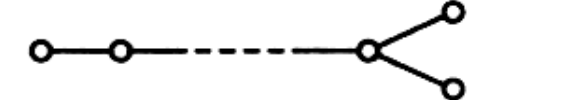
\includegraphics[width=0.24\linewidth]{figures/ch12b-tab1b.png} & 二元二面体群\quad 阶 $=4(n-1)$（$n\geq 4$）\\
  $E_6$ 型 & 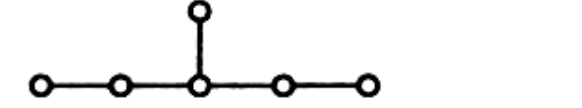
\includegraphics[width=0.24\linewidth]{figures/ch12b-tab1c.png} & 二元四面体群\\
  $E_7$ 型 & 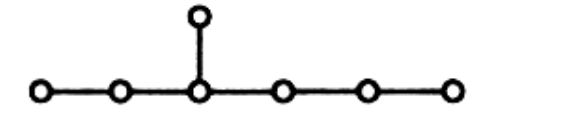
\includegraphics[width=0.24\linewidth]{figures/ch12b-tab1d.png} & 二元八面体群\\
  $E_8$ 型 & 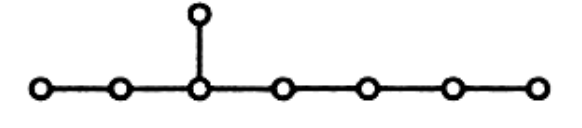
\includegraphics[width=0.24\linewidth]{figures/ch12b-tab1e.png} & 二元二十面体群\\
  \hline
  \end{tabular}
\end{table}

为什么锥形流形奇点消解的 Gromov--Witten 不变量与对称积上 Dirac 算子的等变指数会一致，这非常不可思议；而几何工程真正的论断，是关于结构群 $G$ 未必为 $U(1)$ 的情形。

首先，$4$ 维 Yang--Mills 理论这一侧取 Nekrasov 的配分函数。也就是说，把对称积 $S^n\R^4$ 换成 $G$-半自对偶联络的模空间，同样考虑 Dirac 算子的等变指数。
% [Tutor Note: 原书此处作「$G$-半自己双対接続」，通常称为 $G$-反自对偶联络（$G$-instanton），照录原词并说明。]
另一侧，用来考虑 Gromov--Witten 不变量的非紧 Calabi--Yau 流形则换成别的东西。如后文将说明的，Calabi--Yau 流形上根本看不到结构群 $G$ 的影子。从什么都没有的地方“造出”$G$，才是最不可思议之处，我想这也是它被命名为“工程”的理由。

先回忆：紧 Lie 群 $G$ 由所谓的 Dynkin 图式（见表 1）分类。第 5 章出现的根系也与此相关。例如 $\mathrm{SU}(N)$ 对应 $A_{N-1}$ 型 Dynkin 图式。

另一方面，Coxeter 早已知道 $\mathrm{SL}_2(\C)$ 的有限子群也与 Dynkin 图式对应。设 $\Gamma$ 为 $\mathrm{SL}_2(\C)$ 的有限子群，把 $\C^2/\Gamma$ 在原点处的奇点作奇点消解，所得例外集的不可约分支如何相交，画出来就是 Dynkin 图式。（见表 1 右侧。）这样，有限群 $\Gamma$ 与紧 Lie 群 $G$ 的对应经由分类早已为人熟知；而几何工程把它搬到族上做。最初得到的锥形流形奇点消解 $\cO(-1)\oplus\cO(-1)$ 的各纤维是 $\C^2$，于是让 $\Gamma$ 同样地作用，取商空间 $\cO(-1)\oplus\cO(-1)/\Gamma$。这个空间的奇点消解就是所求的 Calabi--Yau 空间。

% ===== PDF p.167 (原书 p.159) =====
\section{Donaldson--Thomas 不变量}

下面把 Gromov--Witten 不变量与 Donaldson--Thomas 不变量联系起来。这种情形下 Calabi--Yau 流形只需一个，所以某种意义上比前面介绍的不变量之间的等式更简单，也可以说比镜像对称更简单。不过如后文所述，要把两个不变量连起来，在作母函数时必须对所用的变量作解析延拓，这一部分被认为非常困难。

首先粗略说明 Donaldson--Thomas 不变量是什么。要学习准确定义，目前大概只能去读原始论文。

Gromov--Witten 不变量此前数的是从黎曼面 $\Sigma$ 到 $X$ 的全纯映射的“个数”。这里回忆一下本科流形论课程上学到的一条要紧事实：$X$ 中的子流形 $\Sigma$（更准确地说，正规子流形）的定义方式有两种。

\begin{enumerate}[label=\arabic*),leftmargin=2.2em]
\item 是某个流形 $S$ 出发、微分处处单射的嵌入映射 $i:S\to X$ 的像 $\Sigma=i(S)$。
\item 是若干函数（准确地说是局部定义的函数）$f_1,\dots,f_r$ 的公共零点，即 $\Sigma=f_1^{-1}(0)\cap\cdots\cap f_r^{-1}(0)$。
\end{enumerate}

举更简单的例子：要给出 $\R^3$ 中的曲面，可以把曲面参数化，写成
\[
  \Sigma=\{(x(s,t),y(s,t),z(s,t))\mid s,t\in\R\},
\]
也可以给出某个函数 $f$ 写成 $\Sigma=f^{-1}(0)$，有两种方法。作为反函数定理的应用，在像没有奇点的情形，用其中一种方式给出 $\Sigma$，就保证自动也能用另一种方式给出。（不过一般未必能具体写出式子。）

Gromov--Witten 不变量的定义用的是 1) 的参数表示。因为固定定义域的 $\Sigma$，数的正是从 $\Sigma$ 到 $X$ 的全纯映射的个数。
% ===== PDF p.168 (原书 p.160) =====
另一方面，考虑 2) 的理解方式：把全纯映射的像看作函数的公共零点。由于“全纯”，像是复子流形，成为全纯函数的公共零点。于是，与其数全纯映射的个数，不如数全纯函数的公共零点的个数。不过固定一个复子流形 $\Sigma$ 时，以 $\Sigma$ 为公共零点的全纯函数族有多种给法，所以采用代数几何中考虑复子流形时的标准做法：不取 $f_1,\dots,f_r$，而取它们生成的理想。也就是说，把复子流形 $\Sigma$ 与 $X$ 上（准确地说是局部定义的）全纯函数全体 $\cO_X$ 中的理想 $I$ 按
\[
  I=\{f\in\cO_X\mid f|_\Sigma=0\}
\]
对应起来。反之，由理想 $I$，取出它包含的一切函数都取零的点集
\[
  \Sigma=\{x\in X\mid \text{对所有的 } f\in I,\ f(x)=0\},
\]
就能还原 $\Sigma$。不过一般理想对应的集合可能有奇点，需要注意。

这样一来，作为数从 $\Sigma$ 到 $X$ 的全纯映射的个数得到的 Gromov--Witten 不变量的替代，可以考虑数 $X$ 上全纯函数全体中理想的全体。后者正是 Donaldson--Thomas 不变量（的特殊情形）。Gromov--Witten 不变量的情形，按定义域黎曼面的亏格 $g$ 与映射的次数 $\beta\in H_2(X,\Z)$ 作母函数。对理想 $I$，取 Euler 示性数 $\chi(\cO_X/I)$ 代替亏格。
% [Tutor Note: 这里 $\cO_X/I$ 是曲线 $f(C)$ 的结构层，故 $\chi(\cO_X/I)=\chi(\cO_C)=1-g$；亏格 $g$ 的信息就这样被 Euler 示性数吸收。]
若全纯映射 $f:C\to X$ 是嵌入，且 $I$ 是对应于 $f(C)$ 的理想，则 $\chi(\cO_X/I)=1-g$。于是，固定 $n=\chi(\cO_X/I)$ 与 $\beta=[\cO_X/I]$ 的理想模空间记作 $I_n(X,\beta)$，作为 Donaldson--Thomas 不变量的母函数考虑
\begin{equation}
  Z_{DT}(X;q,\Lambda)=\sum_{\beta}\sum_{n}q^n\Lambda^{\beta}\int_{[I_n(X,\beta)]^{\mathrm{vir}}}1
  \tag{4}
\end{equation}
此时，式 (1) 的 $\exp F_{GW}(X;\hbar,\Lambda)$ 与 $Z_{DT}(X;q,\Lambda)$ 在 $q=-e^{i\hbar}$ 的对应下相等，这就是 Maulik--Nekrasov--Okounkov--Pandharipande 猜想。准确地说，需要除掉次数为 0 的部分，这里省略说明，有兴趣的读者请看原始论文。也请再看一遍式 (3)。确实式里能看到变量 $q=-e^{i\hbar}$。

% ===== PDF p.169 (原书 p.161) =====
把子流形的参数表示与函数的公共零点之间的关系想一想，会觉得 Gromov--Witten 不变量与 Donaldson--Thomas 不变量之间似乎有关系，这大概能说得通。但实际作积分时也需要把模空间紧化；而在 DT 一侧并没有与之对应的东西，所以紧化后的模空间相当不同。再者，想一想 $q=-e^{i\hbar}$ 这个变量变换的含义，就会看出它包含若干不可思议的主张。例如式 (1) 在 $\hbar\mapsto-\hbar$ 下不变。若猜想正确，式 (4) 就应在 $q\mapsto1/q$ 这个变量变换下不变。仅看式 (4)，并不明白为什么这种事会成立。而且本来在式 (1) 中 $\hbar$ 是作母函数时的不定元，所以认为 $\hbar$ 接近 0 是自然的；另一方面在式 (4) 中，认为 $q$ 接近 0 才是自然的。因此 $q=-e^{i\hbar}$ 连接的是变量自然定义的位置不同之处。所以这个猜想，无法用逐项检查展开系数是否相等这样的办法来证明。本来这是基于模空间的不变量，所以试图作为模空间之间的关系来理解是自然的，但作解析延拓的部分不落在几何上，因此会走进死胡同。在这个意义上，Gromov--Witten 不变量 $=$ Donaldson--Thomas 不变量这一主张，被认为主张着非常深刻的事情。同样地，自然定义域不同的两个母函数之间通过解析延拓得到的等式，称为 S 对偶性，被认为比镜像对称更深刻。

\section{Donaldson--Thomas 不变量的跨墙公式}

2008 年，Donaldson--Thomas 不变量的研究有了新进展。最后想简单介绍这个。

如第 10 章所说明，在镜像对称的立场上，比起 $X$ 上凝聚层的范畴，其导出范畴 $D(X)$ 被认为更自然。从这样的立场重新审视 Donaldson--Thomas 不变量的定义，就会认为把理想层的模空间 $I_n(X,\beta)$ 推广为参数化导出范畴的对象的模空间更为自然。
% [Tutor Note: 这里的“导出范畴”即 derived category 的中译；原书第 10 章曾用「層の圏」与「導来圏」对举，读者可回看该章。]

% ===== PDF p.170 (原书 p.162) =====
这时成为问题的是，定义模空间时即使固定拓扑数据 $n,\beta$，若把所有对象都考虑进来，就不能指望得到漂亮的空间。这正是代数几何中创立“几何不变量理论”这一分支的动机；从结论来说，必须只取出满足称为稳定性的条件的对象，来作模空间。稳定性条件技术性较强，不易说明；但对理想层的情形，它是从到 $\cO_X$ 的映射为单射这一点自动成立的条件。又因为它是开条件，把稳定对象稍作形变得到的对象仍然稳定。

另外，在考虑导出范畴 $D(X)$ 的对象之前，构造凝聚层模空间时已广为人知：要确定稳定性条件，必须选取 $X$ 上丰沛的线丛或 Kähler 度量。若把它们一般地换掉，稳定的对象可能变得不稳定，因此模空间也随之改变。

进一步，线丛或度量只给出对应于 2 次上同调的部分，所以在导出范畴的情形，必须考虑对应所有次数的上同调群的稳定性条件。这就是 Bridgeland 受物理学家 Douglas 的研究启发而考虑的导出范畴上稳定性条件的空间 $\mathrm{Stab}(D(X))$。
% [Tutor Note: $\mathrm{Stab}(D(X))$ 是 Bridgeland 稳定性条件的参数空间（复流形），其上的“墙”是若干实余维 1 的壁；跨墙公式即比较墙两侧的不变量。]

于是，作为 Donaldson--Thomas 不变量的自然扩张，可以期待如下定义不变量。也就是说，给定稳定性条件 $H\in\mathrm{Stab}(D(X))$，相应地定义参数化 $H$-稳定的 $D(X)$ 对象的模空间 $I^H_n(X,\beta)$，然后在它上面与 (4) 同样地积分 1。

描述换掉这个 $H$ 时不变量如何变化的，就是跨墙公式。2008 年 Kontsevich--Soibelman 给出了它。不过技术上有困难之处，很难认为已给出完全证明，或许说正在完善之中更合适。为什么叫跨墙呢？因为稳定性空间中形成许多墙，只要不越墙不变量就不变，而越墙就会变化。

% ===== PDF p.171 (原书 p.163) =====
实际上，跨墙公式在 4 维流形的 Donaldson 不变量的情形也存在。那是 Göttsche 在 $b_+=1$ 的 4 维流形上，假设 Kotschick--Morgan 猜想成立而证明的，已知它可用自守形式写出。
% [Tutor Note: $b_+$ 是 4 维流形上相交形式正定部分的维数；$b_+=1$ 时 Donaldson 理论的模空间紧化可控，Kotschick--Morgan 猜想才有着落。]
另外，把最近 Göttsche、吉冈与我的共同研究，与望月拓郎的理论结合起来，在射影代数曲面的情形，不假设 Kotschick--Morgan 猜想也证明了出来。分析 $H$ 越墙时哪些对象从稳定变为不稳定，这一点对 Donaldson 不变量和对 Donaldson--Thomas 不变量都很相似。但是目前还不能把两个跨墙公式直接联系起来。从几何工程的角度看，这似乎是有趣的问题。

% 原书作者读音标记［なかじま ひらく］（中島啓）省略，统一按中文版体例处理；本章原书无参考文献表，故不设 reflist。
\renewcommand{\thesection}{\Roman{section}}


